\documentclass[11pt]{article}

\usepackage[a4paper,margin=2.5cm]{geometry}
\usepackage{amsmath,amssymb}
\usepackage{booktabs}
\usepackage{graphicx}
\usepackage{xcolor}
\usepackage{hyperref}
\usepackage{listings}
\usepackage{enumitem}
\usepackage{caption}
\usepackage{parskip}
\usepackage{fancyhdr}
\usepackage{titlesec}
\usepackage{microtype}

\definecolor{codebg}{rgb}{0.96,0.96,0.96}
\definecolor{codekw}{rgb}{0.0,0.2,0.6}
\definecolor{codecom}{rgb}{0.35,0.45,0.35}

\lstset{
  backgroundcolor=\color{codebg},
  basicstyle=\ttfamily\small,
  keywordstyle=\color{codekw}\bfseries,
  commentstyle=\color{codecom}\itshape,
  showstringspaces=false,
  breaklines=true,
  frame=single,
  rulecolor=\color{gray!40},
  xleftmargin=1em,
  xrightmargin=1em,
  aboveskip=8pt,
  belowskip=8pt,
  language=Python,
}

\hypersetup{
  colorlinks=true,
  linkcolor=blue!50!black,
  citecolor=blue!50!black,
  urlcolor=blue!50!black,
  pdftitle={Near-Optimal Space (MGA) Exploration in GreenBubble},
  pdfauthor={GreenBubble project},
}

\titleformat{\section}{\normalfont\Large\bfseries}{\thesection}{0.6em}{}
\titleformat{\subsection}{\normalfont\large\bfseries}{\thesubsection}{0.6em}{}

\pagestyle{fancy}
\fancyhf{}
\fancyhead[L]{\small Near-Optimal Space Exploration in GreenBubble}
\fancyhead[R]{\small\thepage}
\renewcommand{\headrulewidth}{0.3pt}

\title{\textbf{Near-Optimal Space (MGA) Exploration in GreenBubble}\\[4pt]
\large Implementation summary --- what we built, what we reused, and what we would like your feedback on}
\author{GreenBubble project (DTU) \\ prepared for a discussion with Aleksander Grochowicz}
\date{August 2026}

\begin{document}
\maketitle
\thispagestyle{fancy}

\begin{abstract}
\noindent
GreenBubble is a PyPSA-based capacity-expansion model of an industrial
Power-to-X hub (electrolysis, methanolisation, biogas upgrading, storage,
symbiosis). This note summarises how we implemented \emph{Modelling to
Generate Alternatives} (MGA) / near-optimal space exploration on top of it,
following Neumann \& Brown (2021) for the near-optimal space itself and
Grochowicz et al.\ (2023) for the multi-year robustness extension. It is
written for a working discussion: Section~\ref{sec:provenance} is
deliberately explicit about \emph{exactly} what we reused from PyPSA's own
MGA machinery versus what we implemented from scratch, since we did not have
access to a Grochowicz-authored reference implementation and would value
comparing notes.
\end{abstract}

\tableofcontents

% =====================================================================
\section{Motivation}
% =====================================================================
A cost-optimal capacity-expansion solve returns exactly one design. In
practice, many \emph{other} designs are within a few percent of that cost
and can differ substantially in technology mix. Exploring this
\emph{near-optimal feasible space} answers questions the single optimum
cannot: which technologies are load-bearing versus fully substitutable, how
much room exists to steer the design toward secondary goals, and whether one
design stays good across several weather/price years rather than being
over-fitted to the one year it was solved for.

GreenBubble needed this for an additional reason beyond the usual
single-country capacity-expansion setting: it is optimised in two distinct
\emph{modes} --- \texttt{demand} mode (minimise cost to meet fixed product
demands, objective $\geq 0$) and \texttt{price} mode (maximise profit
selling at fixed prices, which shows up in the LP as \emph{minimising} a
cost objective that is typically \emph{negative}, since revenue exceeds
cost). Any near-optimal formulation had to be correct in both regimes, and
also compose with GreenBubble's stochastic (multi-scenario) optimisation
mode. None of this changes the underlying mathematics of Neumann \& Brown or
Grochowicz et al.\ --- it just meant we could not use the reference
formulation completely as-is and had to generalise the sign convention (see
Section~\ref{sec:budget}).

% =====================================================================
\section{Mathematical background}
% =====================================================================

\subsection{The cost-optimal LP and the $\varepsilon$-near-optimal space}
Write the capacity-expansion model as the linear program
\begin{equation}
  \min_{x}\; c^\top x \quad \text{s.t.} \quad Ax \le b,
\end{equation}
where $x$ collects every decision variable (investment \emph{and}
operation), $c^\top x$ is total system cost, and $c_{\mathrm{opt}}$ is its
optimal value. Following Neumann \& Brown (2021) and Grochowicz et al.\
(2023), the \textbf{$\varepsilon$-near-optimal feasible space} is the slice
of the feasible region whose cost is within a relative slack $\varepsilon$
of the optimum:
\begin{equation}
  X_\varepsilon \;=\; \bigl\{\, x : Ax \le b,\;\; c^\top x \le
  (1+\varepsilon)\, c_{\mathrm{opt}} \,\bigr\}.
\end{equation}

\subsection{Sign-robust budget for price-driven (negative-objective) runs}
\label{sec:budget}
GreenBubble adds exactly this extra constraint to the model (the
\emph{budget}), but in a sign-robust form so it also holds when
$c_{\mathrm{opt}} < 0$ (price mode, net revenue):
\begin{equation}
  c^\top x \;\le\; c_{\mathrm{opt}} + \varepsilon\,\lvert c_{\mathrm{opt}}
  \rvert
  \;=\;
  \begin{cases}
    (1+\varepsilon)\, c_{\mathrm{opt}}, & c_{\mathrm{opt}} \ge 0
      \quad \text{(demand mode)} \\[2pt]
    (1-\varepsilon)\, c_{\mathrm{opt}}, & c_{\mathrm{opt}} < 0
      \quad \text{(price mode)}
  \end{cases}
  \label{eq:budget}
\end{equation}
Both branches keep $c_{\mathrm{opt}}$ itself inside the feasible band and
loosen it by the same relative amount $\varepsilon$. Here $c_{\mathrm{opt}}$
is the \emph{optimised LP objective}, \texttt{n.objective} --- not a
re-derived $\text{capex}+\text{opex}$ statistic. For a \textbf{stochastic}
network (PyPSA's multi-scenario mode) it is automatically the
probability-weighted \emph{expected} cost $\sum_s p_s\, c_s^\top x_s$
already, so Eq.~\eqref{eq:budget} defines the near-optimal space
consistently for demand, price, \emph{and} stochastic runs without any
separate scenario-aware bookkeeping.

\subsection{Projection onto technology-capacity dimensions}
Exploring the full-dimensional $X_\varepsilon$ is neither tractable nor
useful for interpretation. We project onto a handful of \emph{technology
capacity} coordinates $y = \sigma(x)$ --- each $y_i$ is the summed installed
capacity of one technology (the $\sigma$-aggregation map of Grochowicz et
al.\ \S 2.2). Exploring a single direction $d$ in this reduced space means
re-solving the original model once with the ordinary cost objective
replaced by $\pm\, d^\top \sigma(x)$, subject to the budget of
Eq.~\eqref{eq:budget} --- this is exactly \emph{Modelling to Generate
Alternatives}.

\subsection{Three tiers}
\begin{description}[leftmargin=1.4em]
  \item[Tier 1 --- ranges.] For each dimension, minimise and maximise it
    alone under the budget: the per-technology min/max installed capacity.
    $\min > 0 \Rightarrow$ \emph{must-have}; $\max \approx 0 \Rightarrow$
    \emph{must-avoid}.
  \item[Tier 2 --- hull.] Sample many search directions $d$ in the selected
    capacity space, solve each, and take the convex hull of the resulting
    extreme points --- the approximated near-optimal polytope.
  \item[Tier 3 --- robustness.] Solve the cost-optimum and explore the hull
    independently for several weather/price years, intersect the resulting
    per-year polytopes, and take the \textbf{Chebyshev centre} (deepest
    interior point) of the intersection as the design that stays
    near-optimal \emph{simultaneously} across all years (Grochowicz et al.\
    \S 2.3--2.4).
\end{description}

\subsection{Shared cost bound and the Chebyshev centre}
For Tier 3, Grochowicz et al.\ (eq.\ 9) note that intersecting per-year
spaces that were each bounded by their \emph{own} optimum $c_{\mathrm{opt}}(i)$
is not directly comparable across years with different absolute cost
levels; a single shared bound
\begin{equation}
  c^\star = \max_i\, c_{\mathrm{opt}}(i)
\end{equation}
can instead be applied to every year's budget, so all years are relaxed
relative to the \emph{same} anchor. GreenBubble exposes this as
\texttt{robustness.cost\_bound: max} (default) versus \texttt{per\_year}.

Given $m$ per-year polytopes (each a \texttt{scipy.spatial.ConvexHull}),
their facet inequalities $a_i^\top y \le b_i$ are stacked into one system;
the Chebyshev centre of the intersection is found via the linear program
\begin{equation}
  \max_{y,\, r}\; r
  \quad \text{s.t.} \quad
  a_i^\top y + r\,\lVert a_i \rVert_2 \le b_i \quad \forall i, \qquad r \ge 0,
\end{equation}
i.e.\ the centre of the largest ball that fits inside every half-space
simultaneously. $r \le 0$ means the per-year near-optimal spaces do not
overlap at all --- itself a meaningful finding (no design is simultaneously
near-optimal in all years at that slack).

% =====================================================================
\section{Implementation architecture}
% =====================================================================
The feature lives in \texttt{scripts/near\_optimal.py} (core algorithms,
$\sim$670 lines), \texttt{scripts/snakemake\_near\_optimal.py} (orchestration
wrapper), the \texttt{explore\_near\_optimal} Snakemake rule, and an
\texttt{mga:} block in \texttt{config.yaml}. It runs \emph{after} a network
is solved --- it consumes the \texttt{*\_OPT.nc} network and never alters
the ordinary solve.

\subsection{Dimension auto-derivation}
A dimension is a technology; its value is the summed installed capacity
(MW) of every \emph{extendable}, \emph{costed} ($\texttt{capital\_cost}>0$)
component belonging to it. The set of selectable dimensions is
\textbf{auto-derived} from the built network --- nothing is hardcoded:
flipping a technology to \texttt{expansion: true} in GreenBubble's own
config automatically makes it available. The grouping key per component is
GreenBubble's own \texttt{comp\_tech\_map} (component name $\to$ technology),
falling back to the PyPSA \texttt{carrier} attribute. The resulting
structure is exactly the nested \texttt{weights} dictionary PyPSA's own MGA
API expects:
\begin{lstlisting}
{tech_key: {"Generator": {"p_nom": {comp_name: 1.0, ...}},
            "Store":     {"e_nom": {comp_name: 1.0, ...}}, ...}}
\end{lstlisting}
Users then pick a small subset (typically 4--5) by name; an unknown name
raises an error listing what is actually available for that network.

\subsection{The constraint-correctness problem}
\label{sec:constraint-problem}
This is the central engineering issue we had to solve, and the reason the
per-direction solve is \emph{not} a direct call to PyPSA's built-in MGA
helpers. GreenBubble adds project-specific custom Linopy constraints to
every ordinary solve (most importantly a maximum
renewable-electricity-to-grid-sales constraint,
\texttt{add\_max\_RE\_sales\_constraint}) via an \texttt{extra\_functionality}
hook. PyPSA's native \texttt{n.optimize.optimize\_mga} /
\texttt{optimize\_mga\_in\_direction} build their \emph{own} model
internally and \textbf{never call \texttt{extra\_functionality}} --- so
using them unmodified would silently drop our custom constraints and compute
the near-optimal space against a \emph{looser}, incorrect feasible region
(higher volumes, wrong must-have/must-avoid flags).

We therefore reproduce PyPSA's own per-direction MGA procedure manually,
step for step, and insert our constraint re-application in the middle:

\begin{lstlisting}
def _solve_mga_in_direction(n, direction, dimensions, c_opt, slack, ...):
    """Constraint-correct replacement for
    n.optimize.optimize_mga_in_direction."""
    m = n.optimize.create_model()                    # <- PyPSA
    cost_objective = m.objective                      # captured before overwrite
    apply_custom_constraints(n, m, n_flags=n_flags,    # <- GreenBubble
                              re_alpha=re_alpha)
    _add_budget_constraint(m, cost_objective,          # <- GreenBubble (Eq. 3)
                            c_opt, slack)

    m.objective = -sum(
        float(direction[k]) *
        n.optimize.build_linexpr_from_weights(dimensions[k], model=m)  # <- PyPSA
        for k in dimensions if direction.get(k, 0)
    )

    status, condition = n.optimize.solve_model(...)   # <- PyPSA
    coords = n.optimize.project_solved(dimensions) if status == "ok" else None
                                                        # <- PyPSA
    return status, condition, coords
\end{lstlisting}
Every Tier-1, Tier-2, and Tier-3 solve funnels through this one function, so
the near-optimal space is always computed against \emph{exactly} the same
feasible region as an ordinary GreenBubble solve.

\subsection{Stochastic-network support}
GreenBubble also supports a PyPSA stochastic (multi-scenario) optimisation
mode, orthogonal to anything in either cited paper. Since the shared
first-stage investment variables ($p_{\mathrm{nom}}$, $e_{\mathrm{nom}}$)
are the same across scenarios, Tiers 1--2 work \emph{transparently} on a
stochastic network once the scenario-broadcast \texttt{(scenario, name)}
MultiIndex on the static component tables is collapsed back to plain
component names (\texttt{is\_stochastic}, \texttt{\_flat\_static}); the MGA
solve itself needs no change since \texttt{n.objective} is already the
expected cost. Tier 3 is deliberately \textbf{skipped} on a stochastic
network: its scenarios already span multiple years/conditions, so
intersecting \emph{again} across years would double-count the same
uncertainty axis.

% =====================================================================
\section{What we reused versus what we wrote from scratch}
\label{sec:provenance}
% =====================================================================
This is the section most relevant to our discussion. We deliberately built
as much as possible on top of \textbf{PyPSA's own native MGA machinery}
(which is Fabian Neumann's reference implementation of Neumann \& Brown
2021, shipped inside PyPSA itself) rather than re-deriving low-level LP
mechanics. \textbf{We did not have access to a Grochowicz-authored code
repository for the 2023 paper} --- our reference for the robustness
extension is the published paper's equations and section numbers only.
Below is an honest, function-level account of provenance.

\subsection{Reused directly via PyPSA's public API (not copied, called)}
\begingroup
\newcommand{\fnbreak}[1]{\allowbreak\texttt{#1}}
\begin{table}[h]
\centering
\small
\begin{tabular}{@{}p{4.7cm}p{2.6cm}p{7.4cm}@{}}
\toprule
\textbf{PyPSA function} & \textbf{Module} & \textbf{Used for} \\
\midrule
\texttt{n}\fnbreak{.optimize}\fnbreak{.create\_model()} & \texttt{pypsa}\fnbreak{.optimization} &
  Building the Linopy LP model for each MGA solve \\
\texttt{n}\fnbreak{.optimize}\fnbreak{.build\_linexpr\_}\allowbreak\texttt{from\_weights()} & \texttt{pypsa}\fnbreak{.optimization} &
  Turning a $\sigma$-weights dict into a Linopy linear expression --- used
  for both the direction objective and Tier 3's ``fix aggregate capacity''
  constraint \\
\texttt{n}\fnbreak{.optimize}\fnbreak{.solve\_model()} & \texttt{pypsa}\fnbreak{.optimization} &
  Solving each direction's LP with the chosen solver/profile \\
\texttt{n}\fnbreak{.optimize}\fnbreak{.project\_solved()} & \texttt{pypsa}\fnbreak{.optimization} &
  Reading solved capacities back, projected onto the selected dimensions \\
\texttt{generate\_directions\_}\allowbreak\texttt{halton}\fnbreak{/evenly\_spaced}\fnbreak{/random()} & \texttt{pypsa}\fnbreak{.optimization}\fnbreak{.mga} &
  Sampling search directions for Tier 2 (used unmodified via a thin
  wrapper) \\
\bottomrule
\end{tabular}
\end{table}
\endgroup

The \texttt{weights} dictionary schema itself (Section~\ref{sec:constraint-problem})
is also PyPSA's own MGA API convention, adopted as-is so our dimension
registry interoperates with these functions without translation.

\subsection{Implemented from scratch (GreenBubble-original)}
\begin{itemize}[leftmargin=1.4em]
  \item \textbf{The manual per-direction solve} (\texttt{\_solve\_mga\_in\_direction}),
    reproducing PyPSA's \texttt{optimize\_mga\_in\_direction} step-by-step
    specifically to insert \texttt{apply\_custom\_constraints} --- the fix
    described in Section~\ref{sec:constraint-problem}. This is the one
    piece of PyPSA-adjacent logic we \emph{did} re-derive, and only because
    the public API leaves no hook to extend it instead.
  \item \textbf{The sign-robust budget} (Eq.~\ref{eq:budget}) generalising
    Neumann \& Brown's $(1+\varepsilon)\,c_{\mathrm{opt}}$ to a
    price-driven, potentially negative objective.
  \item \textbf{Dimension auto-derivation} (\texttt{available\_dimensions},
    \texttt{resolve\_dimensions}) from GreenBubble's own technology config
    and component-to-technology mapping --- no equivalent exists in PyPSA
    or in the cited papers, which assume dimensions are given.
  \item \textbf{Stochastic-network transparency} (Section 3.3) --- an
    extension neither paper addresses, since PyPSA's scenario API postdates
    both.
  \item \textbf{Tier 3 in full}: the shared-bound anchor $c^\star$ (eq.\ 9),
    and the Chebyshev-centre LP itself
    (\texttt{scipy.optimize.linprog} over the stacked hull facet
    inequalities) --- implemented from scratch in Python/NumPy/SciPy
    directly off the paper's \S 2.3--2.4 equations, since no reference code
    was available to adapt.
  \item \textbf{Everything operational around the algorithm}: the
    Snakemake rule and wrapper, the three-tier \texttt{mga:} config block,
    CSV/JSON output schema, and all plotting
    (\texttt{plot\_ranges}, \texttt{plot\_hull\_projections},
    \texttt{plot\_robustness} --- see Section~\ref{sec:results}).
\end{itemize}

\subsection{Verification against the reference implementation}
\label{sec:verification}
While preparing this note we located the official code release for the 2023
paper: \url{https://github.com/aleks-g/intersecting-near-opt-spaces}
(tag \texttt{v1.0.1}, GPL-3.0-or-later, Koen van Greevenbroek \& Aleksander
Grochowicz). We compared our implementation against it directly,
function by function:
\begin{itemize}[leftmargin=1.4em]
  \item \textbf{Chebyshev centre --- confirmed identical.} Their
    \texttt{geometry.ch\_centre()} solves precisely the same LP as our
    \texttt{chebyshev\_centre()}: \mbox{$\max r \text{ s.t. }
    a_i^\top x + r\lVert a_i\rVert \le b_i$} over a hull's
    \texttt{ConvexHull.equations}, same sign handling of the qhull
    convention. We arrived at this independently from the paper's \S 2.4,
    and it matches their reference code exactly. Their version solves the
    LP with Gurobi (\texttt{gurobipy}) directly; ours uses
    \texttt{scipy.optimize.linprog}, a deliberate solver-agnostic choice
    consistent with GreenBubble's documented no-Gurobi-licence fallback path
    (Section~\ref{sec:results}, validation notes) --- same formulation,
    different backend.
  \item \textbf{Shared robustness bound --- confirmed identical.} Their
    \texttt{calc\_obj\_bound.py} computes exactly
    \texttt{obj\_bound = (1 + eps) * max(objs)}, i.e.\ our
    $c^\star = \max_i c_{\mathrm{opt}}(i)$ (eq.\ 9), letter for letter (up
    to our sign-robust $|c_{\mathrm{opt}}|$ generalisation, which their code
    has no analogue for --- their objective is always a positive investment
    cost, never GreenBubble's negative price-mode net revenue).
  \item \textbf{Per-direction MGA solve --- same algorithm, necessarily
    different API.} Their \texttt{utilities}\allowbreak\texttt{.solve\_network\_in\_direction}
    does the same thing ours does (near-optimal budget as an
    \texttt{extra\_functionality} constraint, custom direction objective,
    solve) but against \texttt{pypsa.linopf}/\texttt{linopt} --- PyPSA's
    pre-Linopy optimisation API. GreenBubble runs on PyPSA 1.0.7's Linopy-based
    \texttt{n.optimize} API, which that code cannot run against unmodified;
    our \texttt{\_solve\_mga\_in\_direction} is the same algorithm ported to
    the current API, not a literal reuse.
  \item \textbf{Tier 2 (hull) --- a real, disclosed difference.} Their
    \texttt{compute\_near\_opt.py} is substantially more sophisticated than
    ours: an \emph{adaptive} direction sampler (facet normals of the
    current hull, directions touching the current Chebyshev ball, or both
    combined) with volume- or centre-shift convergence criteria, run until
    convergence or a direction budget is exhausted --- versus our simpler
    fixed-count Halton/random/evenly-spaced sampling via PyPSA's built-in
    generators. Theirs converges to a tighter hull for the same solve
    budget; ours is simpler to reason about and bounded by
    \texttt{n\_directions}. See Section~\ref{sec:dev3} --- closing this gap
    is exactly what we are doing next.
\end{itemize}

\subsection{Reuse plan: \texttt{near-optimal\_dev3}}
\label{sec:dev3}
Their \texttt{geometry.py} module (Chebyshev centre, hull intersection,
facet-normal/hypersphere-based direction sampling) is pure
NumPy/SciPy/(Gurobi) geometry with \textbf{no dependency on the PyPSA
optimisation API} --- unlike the per-direction solve, it does not need
porting to work with GreenBubble's PyPSA version, only the LP backend needs
adapting (Gurobi $\to$ solver-agnostic, as we already do for the Chebyshev
centre). This makes it the practical, low-risk target for direct code
reuse. We are vendoring it on a new \texttt{near-optimal\_dev3} branch:
their geometry utilities are being carried over under their original
GPL-3.0-or-later licence and attribution into a clearly separated module
(rather than merged into GreenBubble's MIT-licensed files, which GPL
licensing does not permit), so that Tier 2's direction sampling and Tier
3's intersection can reuse their adaptive algorithm directly instead of our
simpler from-scratch version --- as much of their code reused as the
licence boundary allows, properly cited.

\subsection{The honest summary}
We reused PyPSA's low-level MGA \emph{mechanics} as much as the public API
allowed, and reimplemented the one piece it doesn't expose a hook for
(constraint-correct solving). Grochowicz et al.\ (2023)'s specific
contribution --- multi-year robustness via intersection and the Chebyshev
centre --- was implemented from the paper's mathematics alone in the current
released version, and Section~\ref{sec:verification} confirms it is
mathematically identical to their reference code where the two are directly
comparable. \textbf{We would value your read on Section~\ref{sec:results}'s
Tier 2 comparison and the \texttt{near-optimal\_dev3} reuse plan above} ---
in particular whether the adaptive sampler's convergence behaviour in
\texttt{compute\_near\_opt.py} has any gotchas we should know about before
we lean on it.

% =====================================================================
\section{Validation status}
% =====================================================================
\begin{itemize}[leftmargin=1.4em]
  \item \textbf{Tier 1 (ranges)}: validated on a synthetic demand-mode
    network, a real deterministic price-mode network
    ($c_{\mathrm{opt}} \approx -60\,\text{M}$, i.e.\ net revenue), and a
    real 3-scenario stochastic price-mode network
    ($c_{\mathrm{opt}} \approx -13.3\,\text{M}$ expected). In every case the
    optimum stayed feasible under its own budget, the custom
    RE-to-grid constraint was confirmed present in the MGA model
    (scenario-aware where relevant), and $\min \le \text{optimal} \le
    \max$ held for every dimension.
  \item \textbf{Tiers 2--3}: validated on synthetic networks (hull geometry,
    intersection/Chebyshev-centre correctness); Tier 2 additionally
    exercised end-to-end on a real network for the tutorial results shown
    in Section~\ref{sec:results}.
  \item \textbf{Solver sensitivity (an operational finding worth
    flagging)}: the MGA objective places weight on only one or two capacity
    variables, so the LP is highly degenerate (many equally-optimal
    vertices). On a real GreenBubble network,
    \texttt{highs-fast} (barrier without crossover) was observed to return
    an outright \emph{infeasible} status with a large primal--dual
    objective error --- silently failing a direction rather than just
    under-reporting its extent. \texttt{gurobi-barrier-fast} did not show
    this failure across 100+ direction solves and remains fast, so it is
    our recommended default; without a Gurobi licence we fall back to a
    profile that terminates at a vertex (\texttt{highs-simplex} /
    \texttt{highs-default}) rather than an interior barrier point.
\end{itemize}

% =====================================================================
\section{Example results (Tutorial 5)}
\label{sec:results}
% =====================================================================
GreenBubble's tutorial 5 (\texttt{tutorials/5\_near\_optimal}) runs all
three tiers end-to-end on a small demonstration network with dimensions
\texttt{[onwind, solar, electrolysis, methanolisation, battery]} at
\texttt{slack = 0.05}. The following figures are produced automatically by
\texttt{scripts/near\_optimal.py}'s plotting functions.

\begin{figure}[h]
  \centering
  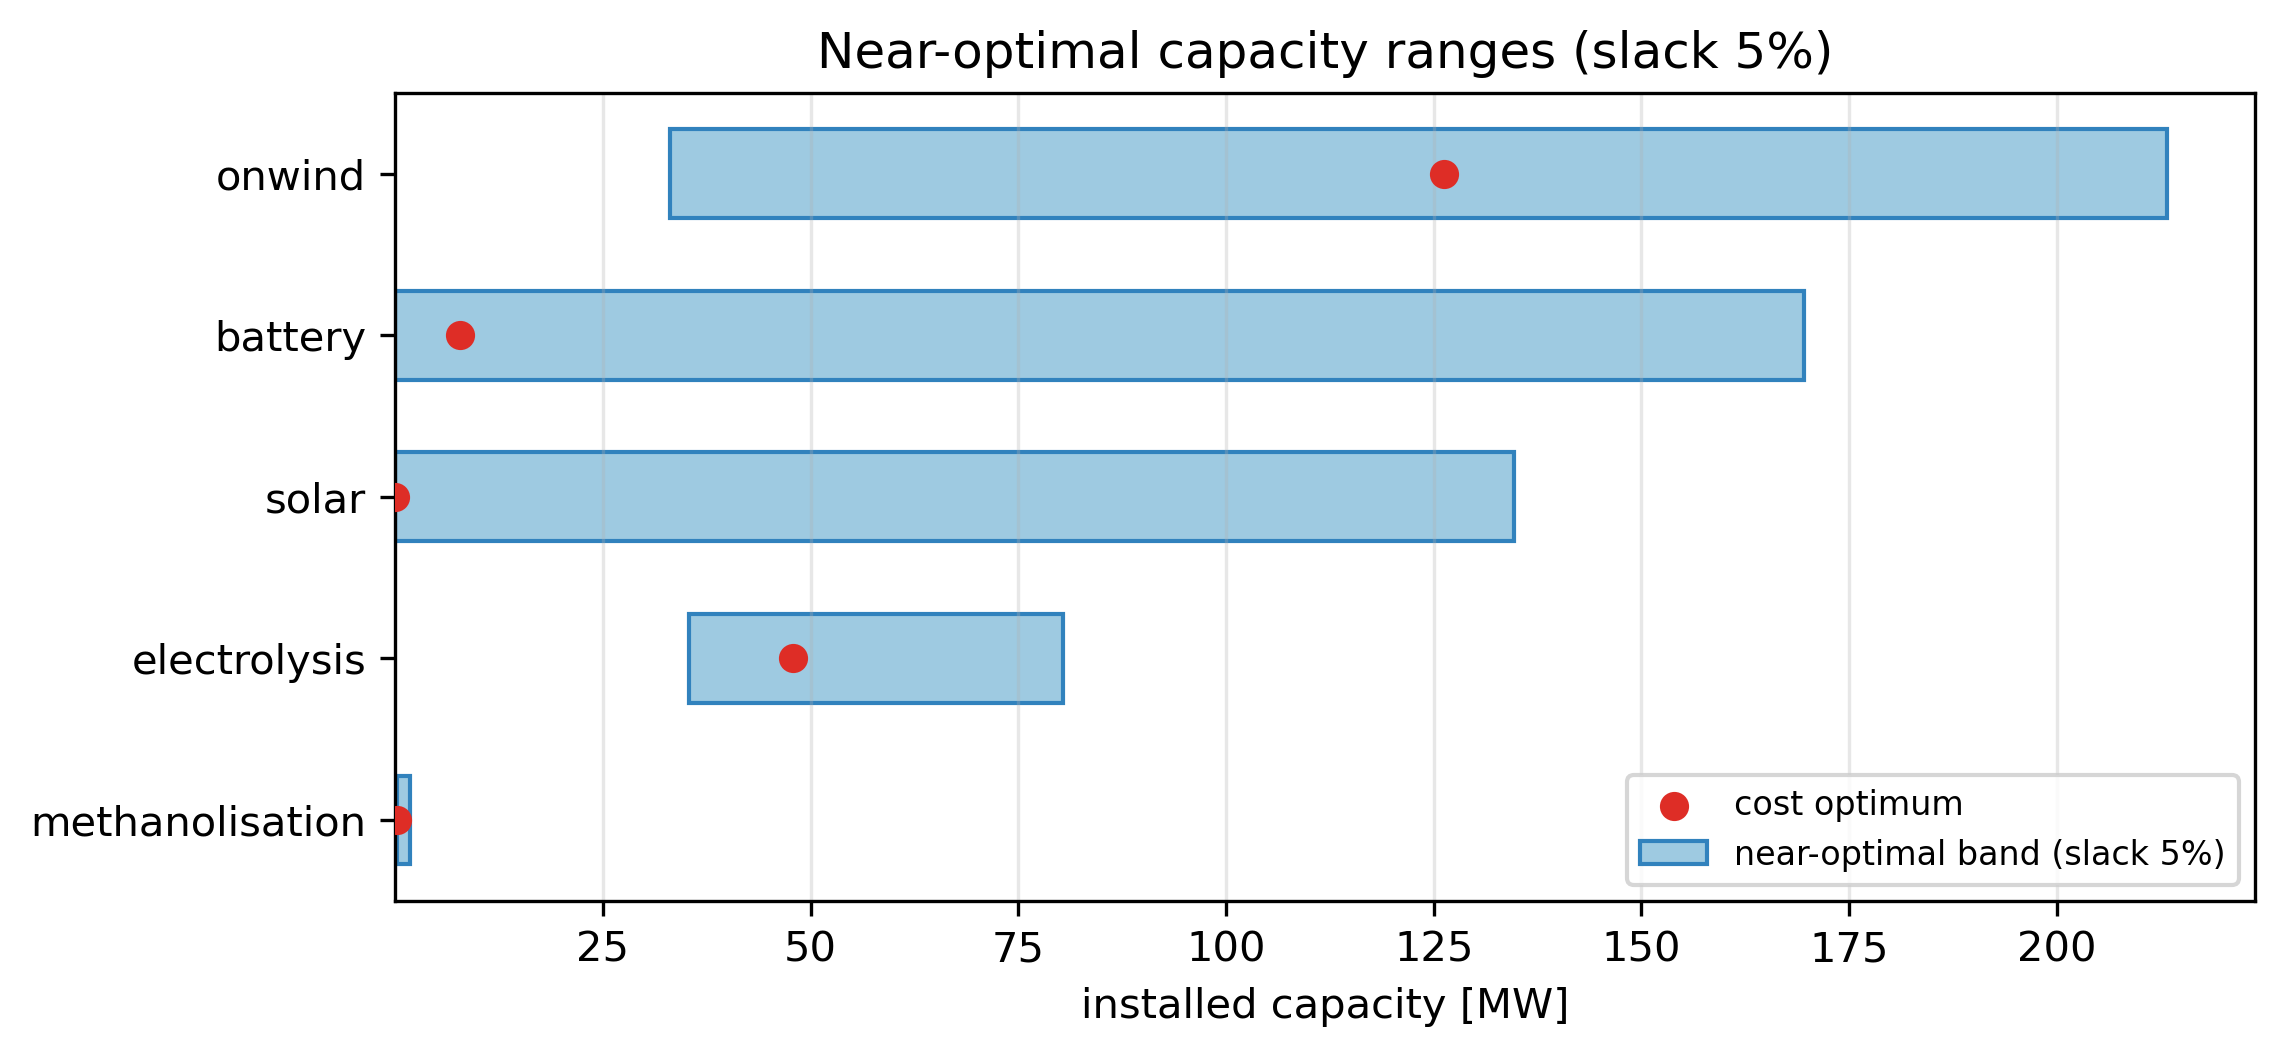
\includegraphics[width=0.85\textwidth]{figures/tut5_nos_ranges.png}
  \caption{Tier 1 --- per-technology near-optimal capacity band (blue) with
  the cost-optimal capacity marked (red). A technology whose band's lower
  bound sits above zero is must-have at this slack; one whose upper bound
  sits at zero is must-avoid.}
\end{figure}

\begin{figure}[h]
  \centering
  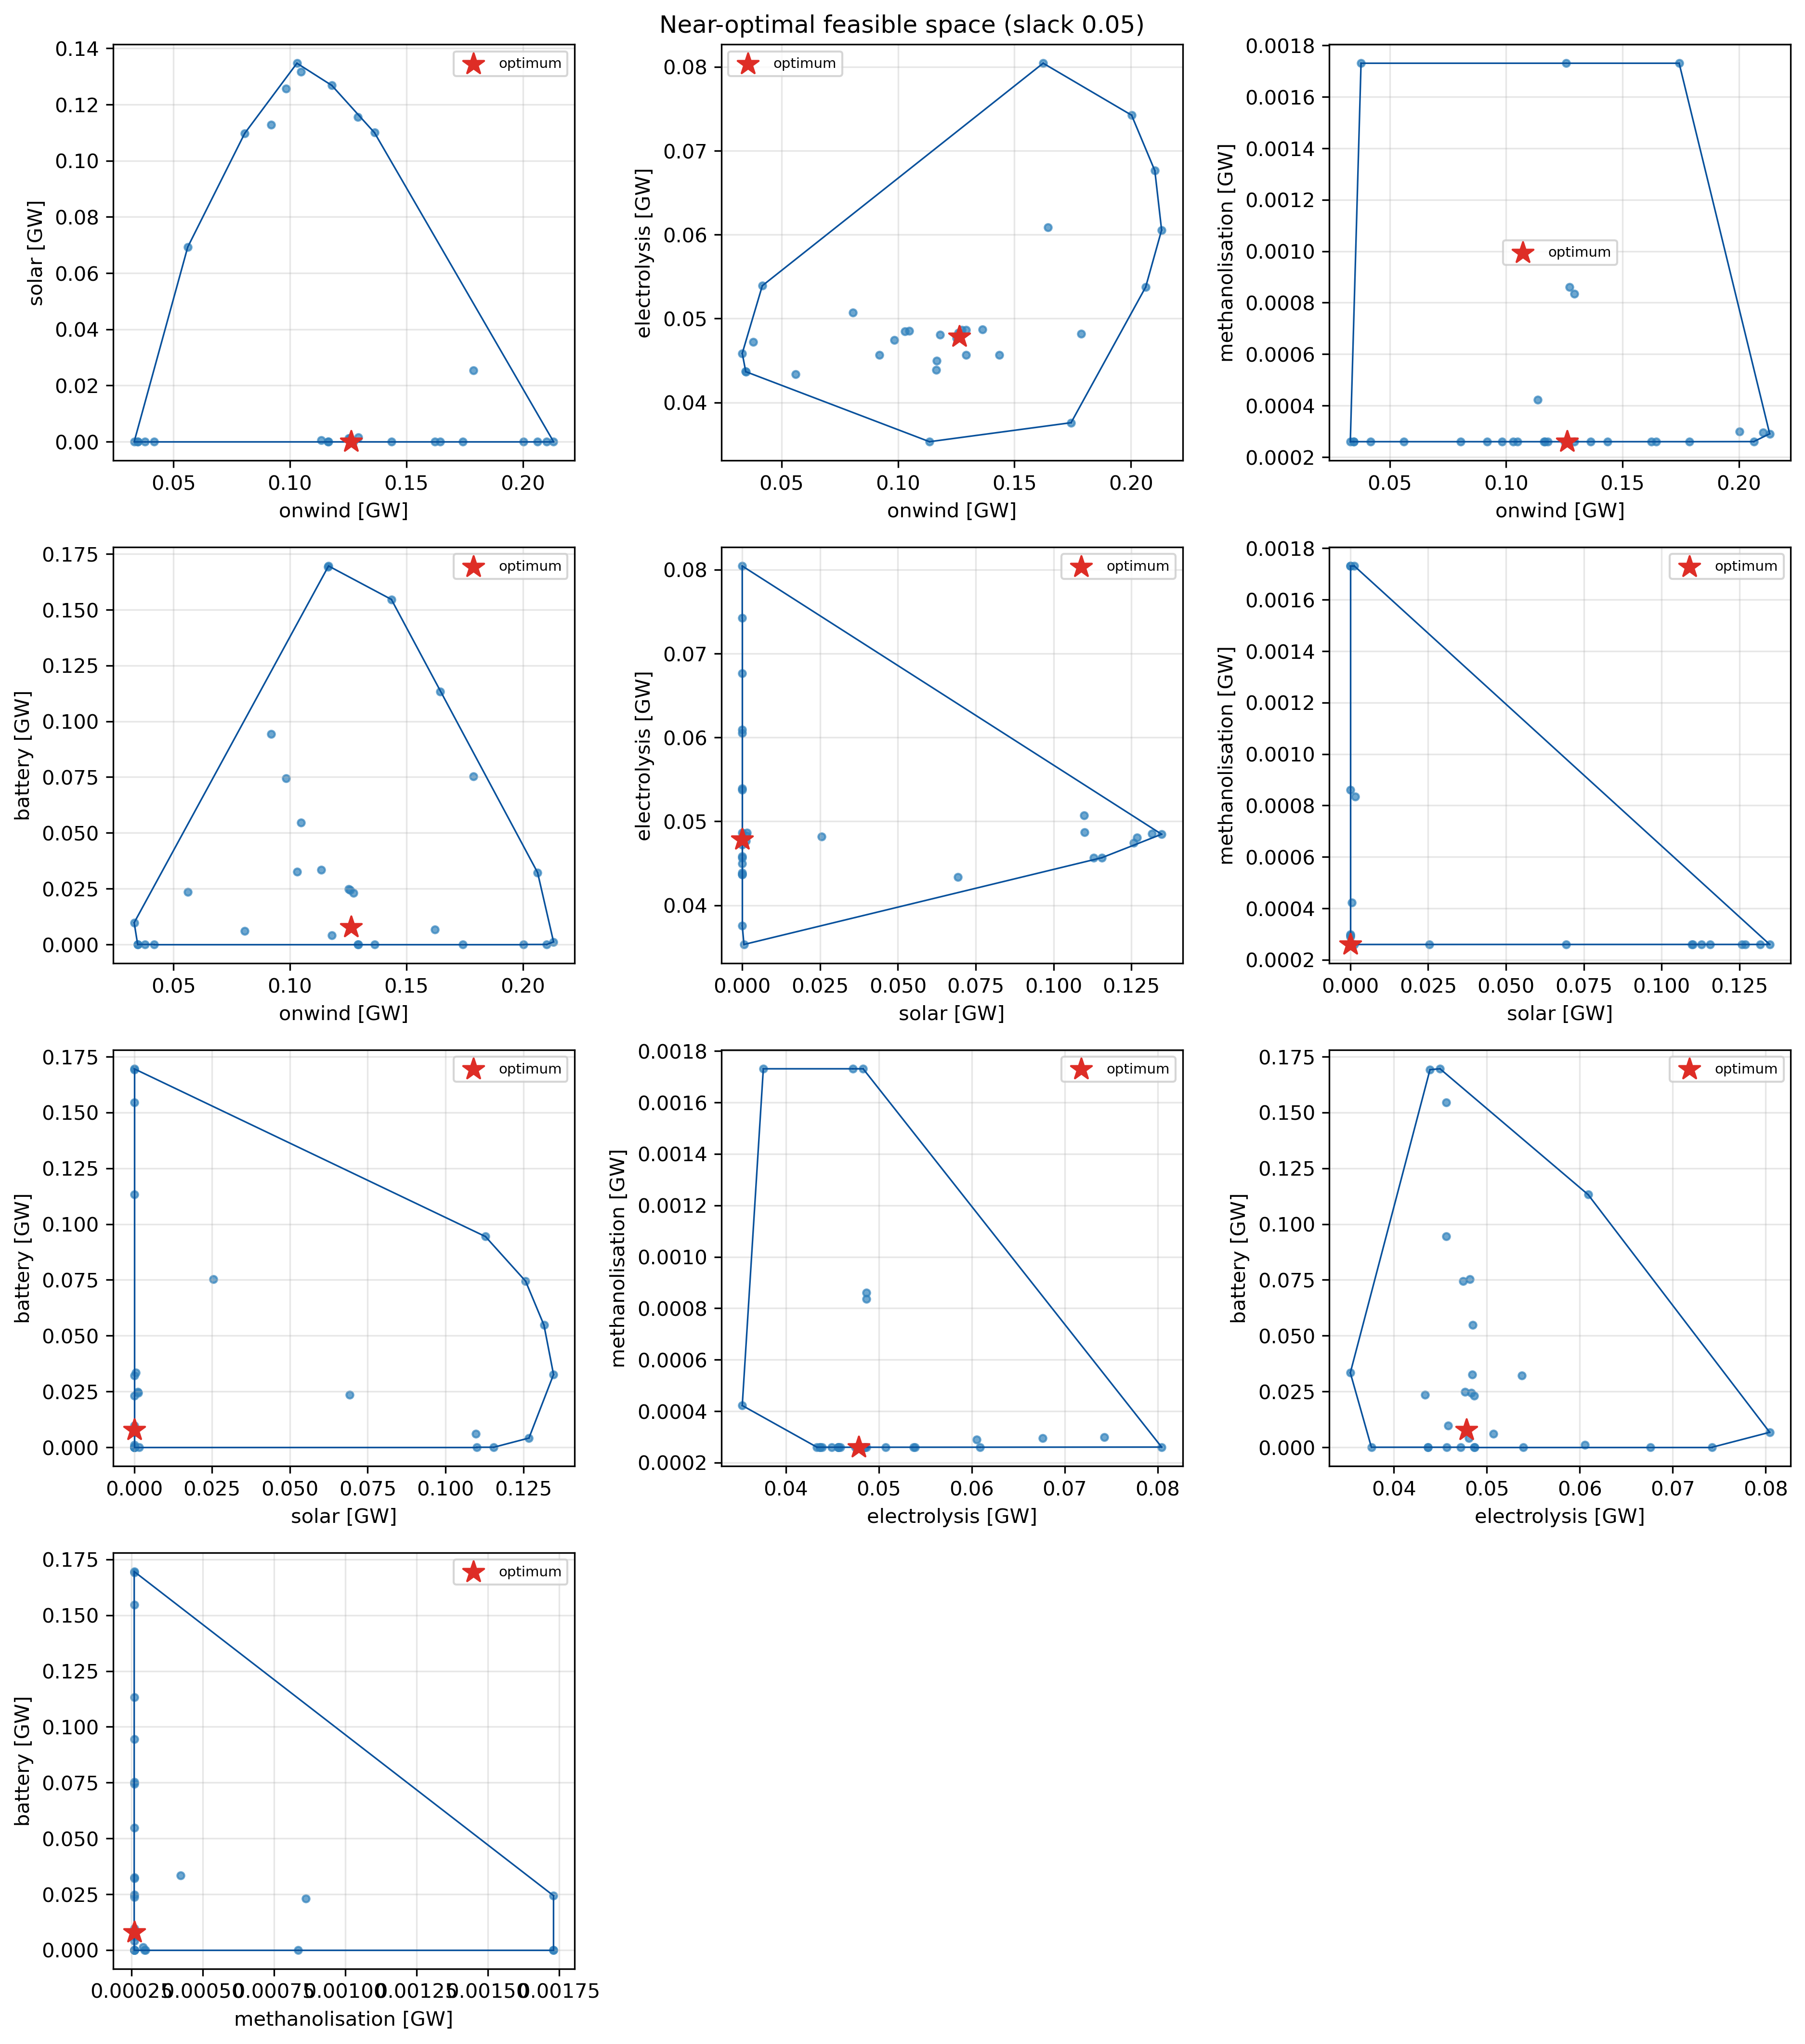
\includegraphics[width=0.95\textwidth]{figures/tut5_nos_hull.png}
  \caption{Tier 2 --- pairwise 2-D projections of the sampled extreme points
  and their convex hull, with the cost optimum marked (red star). Each
  point is one full model solve in a Halton-sampled direction.}
\end{figure}

\begin{figure}[h]
  \centering
  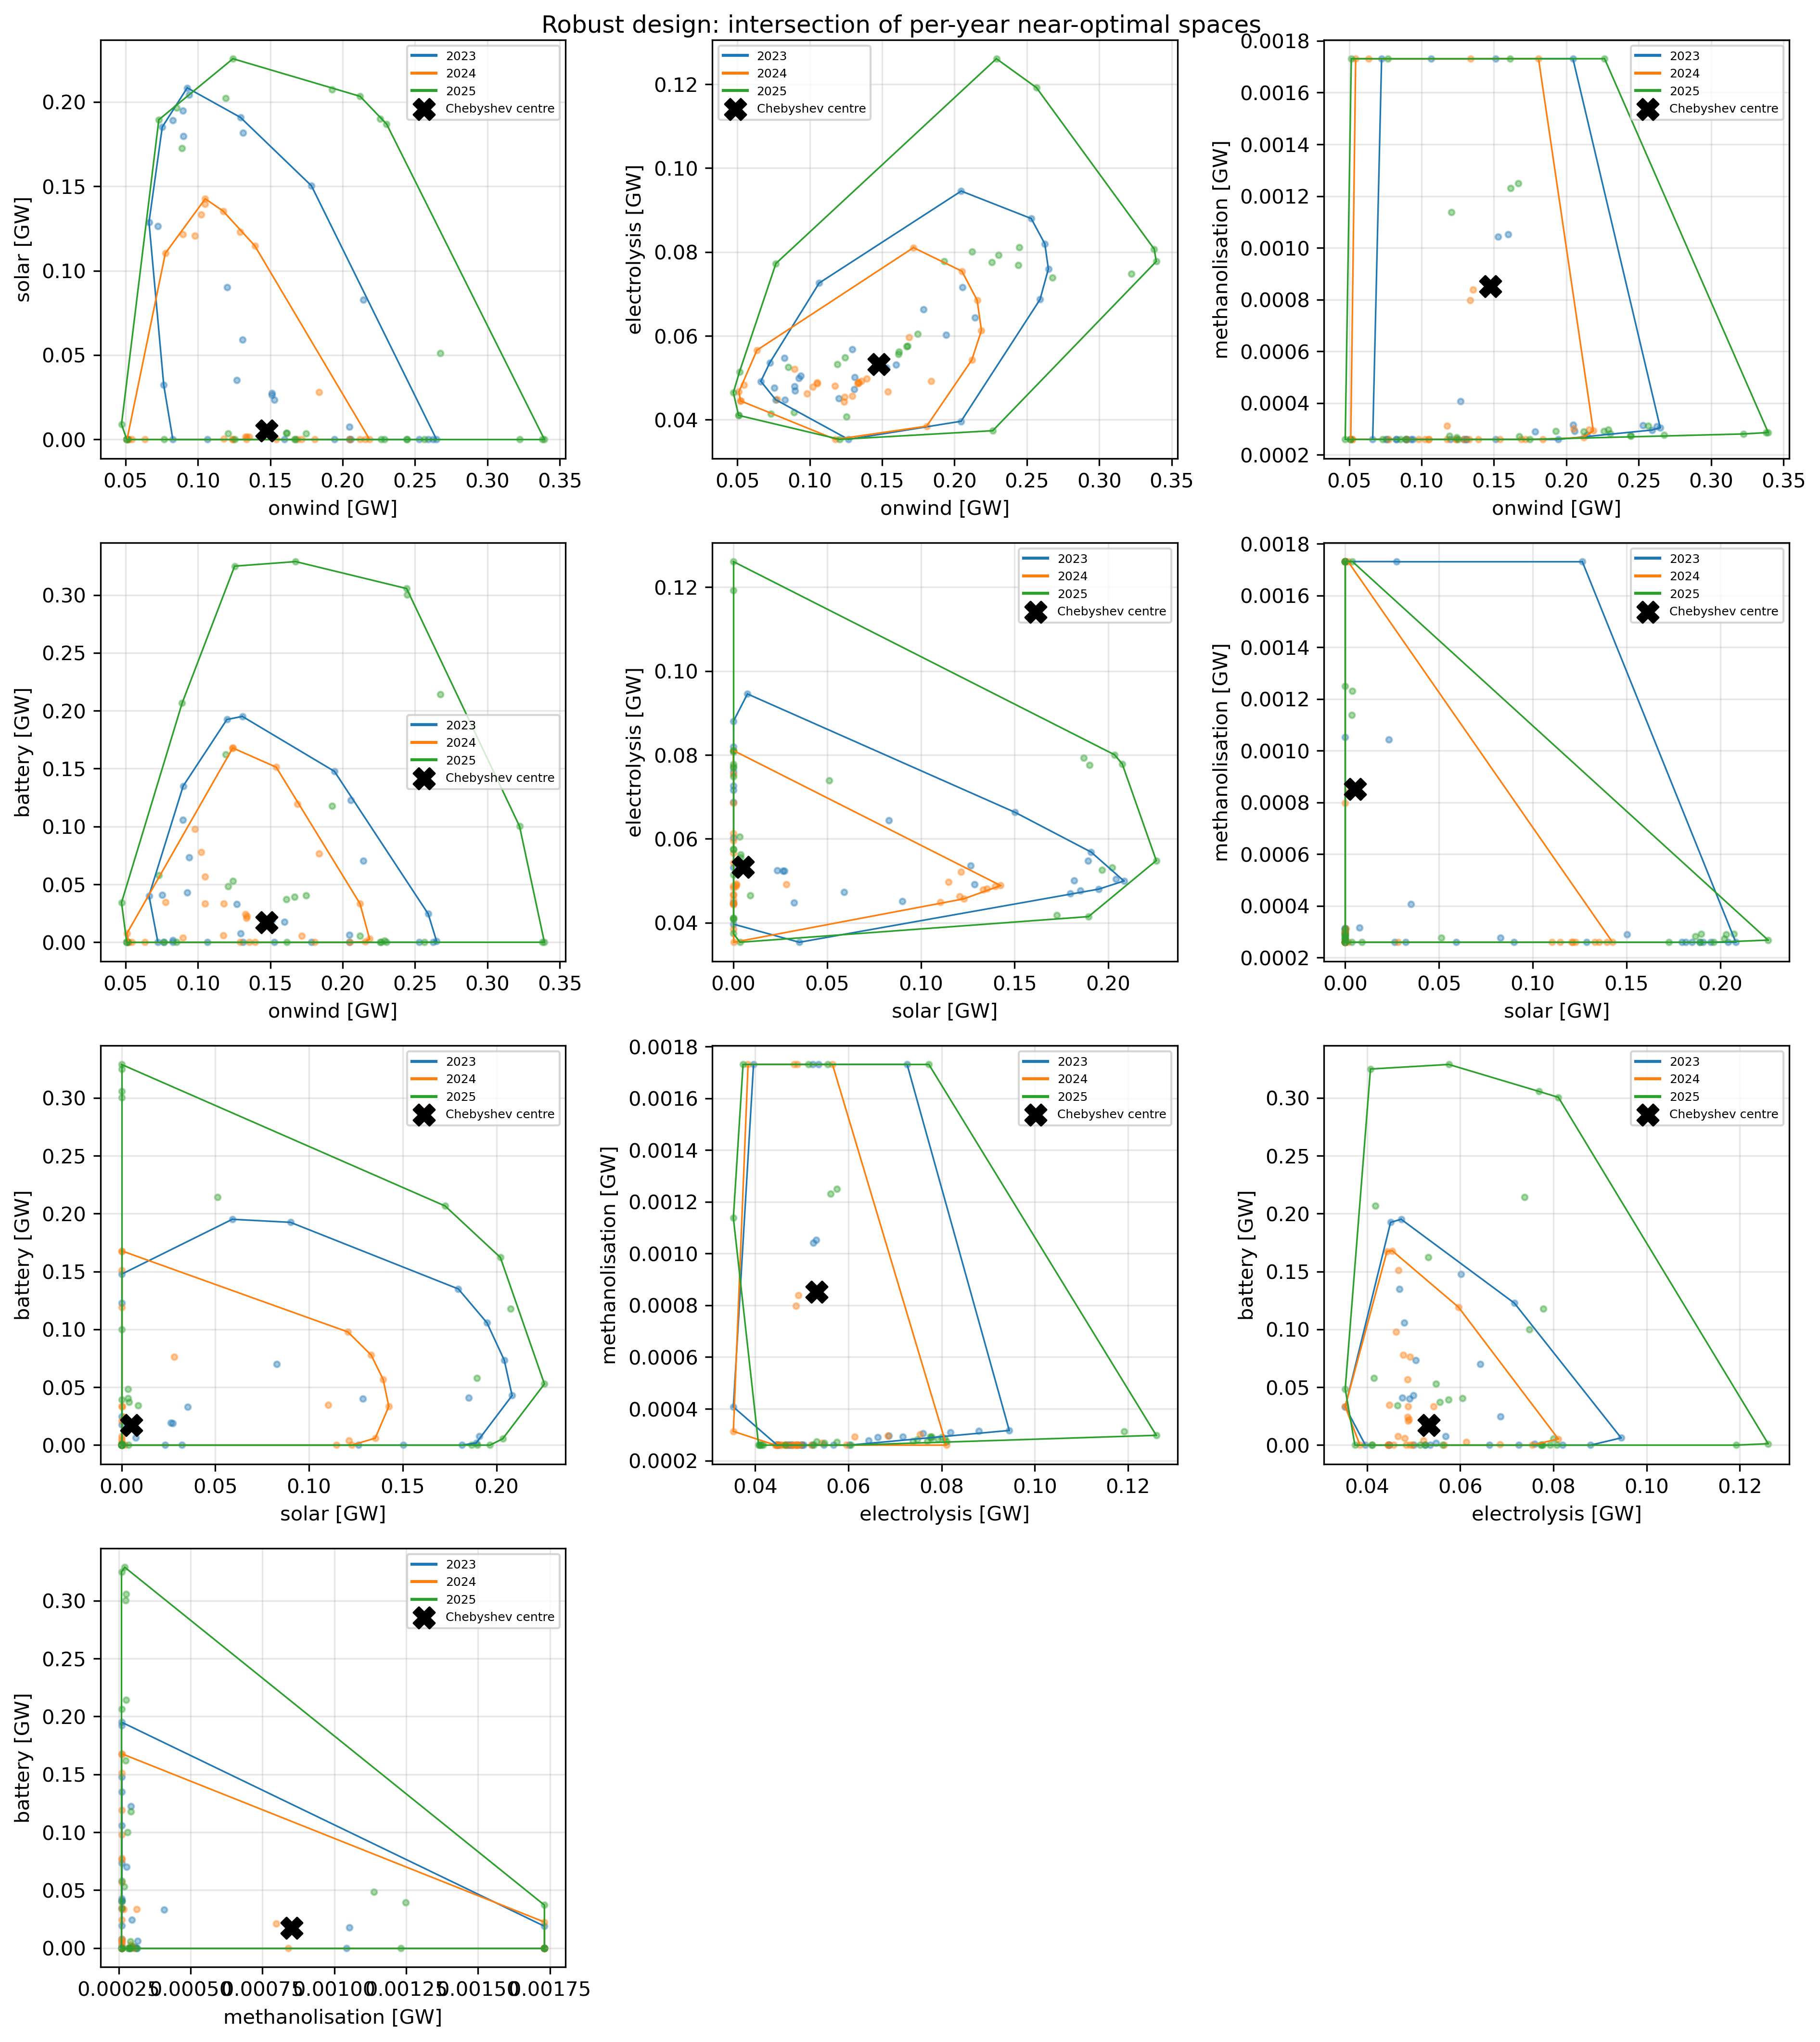
\includegraphics[width=0.95\textwidth]{figures/tut5_nos_robustness.png}
  \caption{Tier 3 --- per-year near-optimal hulls overlaid, with the
  Chebyshev centre of their intersection (black X) as the design that
  stays near-optimal simultaneously across all years explored.}
\end{figure}

\clearpage
% =====================================================================
\section{Discussion points for the meeting}
% =====================================================================
\begin{enumerate}[leftmargin=1.4em]
  \item We're vendoring \texttt{geometry.py}'s adaptive direction sampler
    (facets / touching-ball / combined, with volume- or centre-shift
    convergence) into GreenBubble on a \texttt{near-optimal\_dev3} branch,
    to close the Tier 2 gap in Section~\ref{sec:verification} --- any
    practical gotchas from running it at scale (angle-tolerance tuning,
    typical iteration counts, cases where it stalls) we should know before
    we lean on it?
  \item Does the sign-robust budget generalisation
    (Section~\ref{sec:budget}) for negative-objective (net-revenue,
    price-driven) systems come up in other applications you're aware of?
    We haven't seen it addressed explicitly in either cited paper or in
    the reference code (whose objective is always a positive investment
    cost).
  \item Any feedback on the solver-degeneracy finding in
    Section~\ref{sec:results} (barrier-without-crossover returning
    \emph{infeasible} rather than just an interior point on a highly
    degenerate MGA objective) --- has this come up in your own MGA runs?
    (The reference code always solves via Gurobi's default settings for
    \texttt{ch\_centre}/\texttt{is\_nonempty}, so may not hit this the same
    way.)
  \item How would you extend Tier 3's per-year intersection to compose with
    PyPSA's native \emph{stochastic} (probability-weighted scenario) mode,
    which we currently treat as orthogonal (Tier 3 skipped on stochastic
    networks, see Section 3.3) rather than combined?
\end{enumerate}

% =====================================================================
\section*{References}
% =====================================================================
\begin{itemize}[leftmargin=1.4em]
  \item Neumann, F. \& Brown, T. (2021). \emph{The Near-Optimal Feasible
    Space of a Renewable Power System Model}. Electric Power Systems
    Research, 190, 106690.
    \url{https://doi.org/10.1016/j.epsr.2020.106690}
    (\href{https://arxiv.org/abs/1910.01891}{arXiv:1910.01891})
  \item Grochowicz, A., van Greevenbroek, K., Benth, F.E. \& Zeyringer, M.\
    (2023). \emph{Intersecting Near-Optimal Spaces: European Power Systems
    with More Resilience to Weather Variability}. Energy Economics.
    \url{https://doi.org/10.1016/j.eneco.2022.106496}
    (\href{https://arxiv.org/abs/2206.12242}{arXiv:2206.12242})
  \item PyPSA MGA documentation:
    \url{https://docs.pypsa.org/latest/user-guide/optimization/modelling-to-generate-alternatives/}
  \item van Greevenbroek, K. \& Grochowicz, A. Reference implementation for
    the 2023 paper. \url{https://github.com/aleks-g/intersecting-near-opt-spaces}
    (tag \texttt{v1.0.1}, GPL-3.0-or-later).
  \item GreenBubble docs: \texttt{docs/guide\_near\_optimal.rst},
    \texttt{docs/tutorial\_5\_near\_optimal.rst},
    \texttt{scripts/near\_optimal.py} (implementation),
    \texttt{scripts/snakemake\_near\_optimal.py} (orchestration).
\end{itemize}

\end{document}
